%% abtex2-modelo-relatorio-tecnico.tex, v<VERSION> laurocesar
%% Copyright 2012-<COPYRIGHT_YEAR> by abnTeX2 group at http://www.abntex.net.br/ 
%%
%% This work may be distributed and/or modified under the
%% conditions of the LaTeX Project Public License, either version 1.3
%% of this license or (at your option) any later version.
%% The latest version of this license is in
%%   http://www.latex-project.org/lppl.txt
%% and version 1.3 or later is part of all distributions of LaTeX
%% version 2005/12/01 or later.
%%
%% This work has the LPPL maintenance status `maintained'.
%% 
%% The Current Maintainer of this work is the abnTeX2 team, led
%% by Lauro César Araujo. Further information are available on 
%% http://www.abntex.net.br/
%%
%% This work consists of the files abntex2-modelo-relatorio-tecnico.tex,
%% abntex2-modelo-include-comandos and abntex2-modelo-references.bib
%%

% ------------------------------------------------------------------------
% ------------------------------------------------------------------------
% abnTeX2: Modelo de Relatório Técnico/Acadêmico em conformidade com 
% ABNT NBR 10719:2015 Informação e documentação - Relatório técnico e/ou
% científico - Apresentação
% ------------------------------------------------------------------------ 
% ------------------------------------------------------------------------

\documentclass[
	% -- opções da classe memoir --
	12pt,				% tamanho da fonte
	a4paper,		% tamanho do papel. 
	oneside,    % remover paginas em branco
	% -- opções da classe abntex2 --
	chapter=TITLE,		   % títulos de capítulos convertidos em letras maiúsculas
	section=TITLE,		   % títulos de seções convertidos em letras maiúsculas
	subsection=TITLE,	   % títulos de subseções convertidos em letras maiúsculas
	subsubsection=TITLE, % títulos de subsubseções convertidos em letras maiúsculas
	% -- opções do pacote babel --
	english,			% idioma adicional para hifenização
	french,				% idioma adicional para hifenização
	spanish,			% idioma adicional para hifenização
	brazil,				% o último idioma é o principal do documento
]{abntex2}


% ---
% PACOTES
% ---

%--
% Modificações
\usepackage{./latex/ence}

% ---
% Pacotes fundamentais 
% ---
%\usepackage{lmodern}			% Usa a fonte Latin Modern
\usepackage[T1]{fontenc}		% Selecao de codigos de fonte.
\usepackage[utf8]{inputenc}		% Codificacao do documento (conversão automática dos acentos)
\usepackage{indentfirst}		% Indenta o primeiro parágrafo de cada seção.
\usepackage{color}				% Controle das cores
\usepackage{graphicx}			% Inclusão de gráficos
\usepackage{microtype} 			% para melhorias de justificação
% ---

% ---
% Pacotes adicionais, usados no anexo do modelo de folha de identificação
% ---
\usepackage{multicol}
\usepackage{multirow}
% ---

% ---
% Pacotes de citações
% ---
\usepackage[brazilian,hyperpageref]{backref}	 % Paginas com as citações na bibl
\usepackage[alf]{abntex2cite}	% Citações padrão ABNT

% ---
% Pacote para que imagens e tabelas não mudem de lugar
% ---
\usepackage{float}
\floatplacement{figure}{H}
\floatplacement{table}{H}

% ---
% Informações de dados para CAPA e FOLHA DE ROSTO
% ---
\titulo{Optimização Bayesiana}
\autor{Douglas Martins Mendes Braga\\
Felipe Sales}
\local{Rio de Janeiro}
\data{2020}
\instituicao{Instituto Brasileiro de Geografia e Estatística - IBGE

Escola Nacional de Ciências Estatísticas - ENCE

Bacharelado em Estatística}
\orientador{aaaaaaaaaa}
\coorientador{lalalala}
\preambulo{Monografia apresentada à Escola Nacional de Ciências Estatísticas do
Instituto Brasileiro de Geografia e Estatística como requisito parcial à
obtenção do título de Bacharel em Estatística.}
% ---

% ---
% Configurações de aparência do PDF final

% informações do PDF
\makeatletter
\hypersetup{
	  colorlinks=false,      		% false: boxed links; true: colored links
	  bookmarksdepth=4
}
\makeatother
% --- 

% --- 
% Espaçamentos entre linhas e parágrafos 
% --- 

% O tamanho do parágrafo é dado por:
\setlength{\parindent}{1.3cm}

% Controle do espaçamento entre um parágrafo e outro:
\setlength{\parskip}{0.2cm}  % tente também \onelineskip

% Seleciona o idioma do documento (conforme pacotes do babel)
\selectlanguage{brazil}

% Retira espaço extra obsoleto entre as frases.
\frenchspacing 

%\usepackage{fontspec}
%\setmainfont{Calibri}

%
\usepackage{caption}
\captionsetup[figure]{
    position=above,
}

% ----
% Início do documento
% ----
\begin{document}

% ----------------------------------------------------------
% ELEMENTOS PRÉ-TEXTUAIS
% ----------------------------------------------------------
\pretextual

% ---
% compila o indice
% ---
\makeindex
% ---

% ---
% Capa
% ---
\imprimircapa
% ---

% ---
% Folha de rosto
% (o * indica que haverá a ficha bibliográfica)
% ---
\imprimirfolhaderosto*


% ------------------
% Folha de aprovação
%-------------------
\imprimitfolhadeaprovacao

% ---
% Agradecimentos
% ---
\begin{agradecimentos}
  O agradecimento principal é direcionado a Youssef Cherem.
  
  Os agradecimentos especiais são direcionados ao Centro de Pesquisa em
  Arquitetura da Informação\footnote{\url{http://www.cpai.unb.br/}} da
  Universidade de Brasília (CPAI), ao grupo de usuários
  \emph{latex-br}\footnote{\url{http://groups.google.com/group/latex-br}}
  e aos novos voluntários do grupo
  \emph{\abnTeX}\footnote{\url{http://groups.google.com/group/abntex2} e
  \url{http://www.abntex.net.br/}}\textasciitilde{}que contribuíram e que
  ainda contribuirão para a evolução do abn\TeX.
\end{agradecimentos}
% ---

% ---
% RESUMO
% ---

% resumo na língua vernácula (obrigatório)
\setlength{\absparsep}{18pt} % ajusta o espaçamento dos parágrafos do resumo
\begin{resumo}
 O resumo deve ressaltar o objetivo, o método, os resultados e as
 conclusões do documento. A ordem e a extensão destes itens dependem do
 tipo de resumo (informativo ou indicativo) e do tratamento que cada item
 recebe no documento original. O resumo deve ser precedido da referência
 do documento, com exceção do resumo inserido no próprio documento.
 (\ldots) As palavras-chave devem figurar logo abaixo do resumo,
 antecedidas da expressão Palavras-chave:, separadas entre si por ponto e
 finalizadas também por ponto.
 \noindent
 \\
 \\
 \textbf{Palavras-chaves}: Otimização. Estatística Bayesiana. Machine Learning.
\end{resumo}
% ---

% ---
% inserir lista de ilustrações
% ---
\pdfbookmark[0]{\listfigurename}{lof}
\listoffigures*
\clearpage
% ---

% ---
% inserir lista de tabelas
% ---
\pdfbookmark[0]{\listtablename}{lot}
\listoftables*
\clearpage
% ---

% ---
% inserir o sumario
% ---
\pdfbookmark[0]{\contentsname}{toc}
\tableofcontents*
\clearpage
% ---

% ----------------------------------------------------------
% ELEMENTOS TEXTUAIS
% ----------------------------------------------------------
\textual
\pagestyle{plain}

\hypertarget{introduuxe7uxe3o}{%
\chapter{Introdução}\label{introduuxe7uxe3o}}

Os algoritmos de Machine Learning raramente não possuem parãmetros, como
por exemplo, a taxa de aprendizado. Muitas vezes esses parâmetros são
definidos por tentativa e erro.

A optimização bayesiana é um método para encontrar pontos próximos a
pontos ótimos das funções, esta técnica utiliza-se de suposições a
priori e combina com evidências dos dados para obter a posteriori. ~

\begin{table}

\caption{\label{tab:unnamed-chunk-8}Iris}
\centering
\begin{tabular}[t]{r|r|r|r|l}
\hline
Sepal.Length & Sepal.Width & Petal.Length & Petal.Width & Species\\
\hline
5.1 & 3.5 & 1.4 & 0.2 & setosa\\
\hline
4.9 & 3.0 & 1.4 & 0.2 & setosa\\
\hline
4.7 & 3.2 & 1.3 & 0.2 & setosa\\
\hline
4.6 & 3.1 & 1.5 & 0.2 & setosa\\
\hline
5.0 & 3.6 & 1.4 & 0.2 & setosa\\
\hline
\multicolumn{5}{l}{\textit{Fonte: } O próprio autor}\\
\end{tabular}
\end{table}

lalalalal

\hypertarget{revisuxe3o-de-literatura}{%
\chapter{Revisão de Literatura}\label{revisuxe3o-de-literatura}}

\hypertarget{base-de-dados}{%
\chapter{Base de Dados}\label{base-de-dados}}

\hypertarget{metodologia}{%
\chapter{Metodologia}\label{metodologia}}

\hypertarget{otimizauxe7uxe3o}{%
\section{Otimização}\label{otimizauxe7uxe3o}}

Um problema de otimização pode ser definido como:

\[
\mbox{maximize } f(x)
\]

\[
\mbox{restrito a } \boldsymbol{x} \leq \boldsymbol{\Omega}
\]

Esse é um caso de otimização onde busca-se o maior valor possível da
função objetivo \(f\) tendo \(\Omega\) como as restrições desta
otimização e \(\boldsymbol{x} = (x_1,...,x_n)\) como o vetor das
variáveis independentes.\footnote{Chong and Zak (2013)}

Porém, normalmente pressupõe-se que a função objetivo tem uma
representação matemática conhecida, é convexa ou pelo menos é facilmente
avaliada. No campo de Machine Learning, uma parte das funções de custo
estudadas não seguem nenhuma dessas suposições e além disto, muitas
vezes, a avaliação da função é muito custosa(demorada), e as propriedas
da função objetivo são desconhecidas e as vezes.\\

\hypertarget{inferuxeancias-bayesiana}{%
\section{Inferências Bayesiana}\label{inferuxeancias-bayesiana}}

\hypertarget{processos-gaussianos}{%
\section{Processos Gaussianos}\label{processos-gaussianos}}

Os processos gaussianos comumente são utilizados como para interpolação
de pontos não linear, sendo assim, o objetivo é prever pontos no espaço
não observados, levando em conta que pontos próximos aos observados não
devem mudar bruscamente o valor da variável de interesse. Abaixo será
apresentado um exemplo.\\

\begin{figure}
\centering
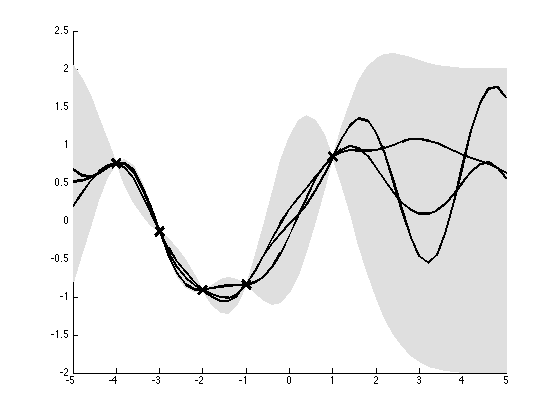
\includegraphics[width=\textwidth,height=0.3\textheight]{fig/gp.png}
\caption{\href{https://github.com/probml/pmtk3/blob/30d7a1952f3979b16e92dbfa4cd1ce0e402cf7d8/docs/demoOutput/bookDemos/(15)-Gaussian_processes/gprDemoNoiseFree_02.png}{Retirada
do livro de Kevin Murphy.\label{gp}}}
\end{figure}

Na figura \ref{gp} pode-se observar, que neste caso, esta sendo
considerado que não há incerteza de medição nos pontos observados
represetados pelo \(x\) no gráfico, as bandas representam um intervalo
de confiança de 95\%.\\

Para o entendimento dos processos gaussianos é necessário que seja
definido uma noção de similaridade e de variância'

Os processos gaussinaos também podem ser utilizados como distribuição a
priori para uma conjunto de pontos no espaço.\\

Pode-se imaginar como exemplo \(n\) ponto gerados de uma distribuição
n-dimensional normal multivariada, agora imaginando pontos de um domínio
contínuo tem-se um processo gaussiano sendo a generalização
infinito-dimensional de uma variável multi-dimensional gaussiana.\\

A optimização bayesiana utiliza como priori o Processo Gaussiano com o
vetor de médias 0 para facilitar as contas, porém, um fato interessante
do processo gaussiano é que este pode ser totalmente definido pela sua
matriz de covariância.\footnote{Bishop (2012)}\\

A matriz de covariância de um processo gaussiano depende de qual
kernel(K) será utilizado, um dos mais utilizado é o gaussiano, que
possui este nome por ter o mesmo formato da distribução
normal(gaussiana) tendo como única diferença a constnate de
normalização, definido a seguir.\\

\[
X \sim GP(0,\Sigma)
\]

\[
\Sigma(x_1,x_2) = K(x_1,x_2) + I\sigma^2_y
\]

\[
K(x_1,x_2) = \sigma^2 e^{-\frac{1}{2l^2}(x_1-x_2)^2}
\]

Será assumido que a função \(f(x)\) é uma observação de um processo
gaussiano e que as observações, \((x_n,y_n)_{n=1}^N\), onde
\(y_n \mbox{~} N(f(x_n),\nu)\) e \(\nu\) é a variância dos ruídos
introduzidos na função de observação. Utilizando a regra de bayes para
combinar a proiri com os dados para gerar a posteriori que determina
qual ponto de \(\chi\)

\hypertarget{otimizauxe7uxe3o-bayesiana}{%
\section{Otimização Bayesiana}\label{otimizauxe7uxe3o-bayesiana}}

A optimização bayesiana é útil quando a avaliação da função tem custo
alto, quando não é conhecido as derivadas da função em análise, quando a
função não é convexa ou até mesmo desconhecida.\\

As técnicas de otimização bayesiana são algumas das abordagens mais
eficientes em termos do número de avaliações de funções necessárias. É
conhecida com este nome por ter como base o teorema de Bayes que diz que
a posteriori de um modelo(M) dada evidência dos dados(E) é proporcional
à verossimilhança de E dado M vezes a priori do modelo(M):

\[
P(M|E) \propto P(E|M)P(M)
\]

Na optimização bayesiana, a priori que é definida está ligada ao espaço
que acredita-se que a função de custo possa variar. Mesmo que esta
função seja desconhecida, é razoavel supor que exista conhecimento
prévio sobre alguma de suas propriedades, como a suavidade, isto torna
algumas funções objetivas mais prováveis que outras.\\

Define-se \(x_i\) sendo a i-ésima amostra, e \(f(x_i)\) a observação da
função objetiva em \(x_i\). Serão acumulados as observações
\(D_{i:t}=\left\{ x_{i:t},f(x_{1:t}) \right\}\), a distribuição apriori
será combinada com a verossimilhança \(P(D_{i:t}|f)\), que para
facilitar, pode-se pensar que a verossimilhança é a proprabilidade do
que vimos ocorrer dado que o que achamos sobre a função é a realidade.
Se a nossa crença anterior é que a função objetiva é muito suave e
isenta de erros, os dados com alta variância ou oscilações devem ser
considerados menos prováveis do que os dados que mal se desviam da
média. Agora, podemos combiná-los para obter nossa distribuição
aposteriori:

\[
P(f|D_{1:t}) \propto P(D_{1:t}|f)P(f)
\]

\begin{figure}
\centering
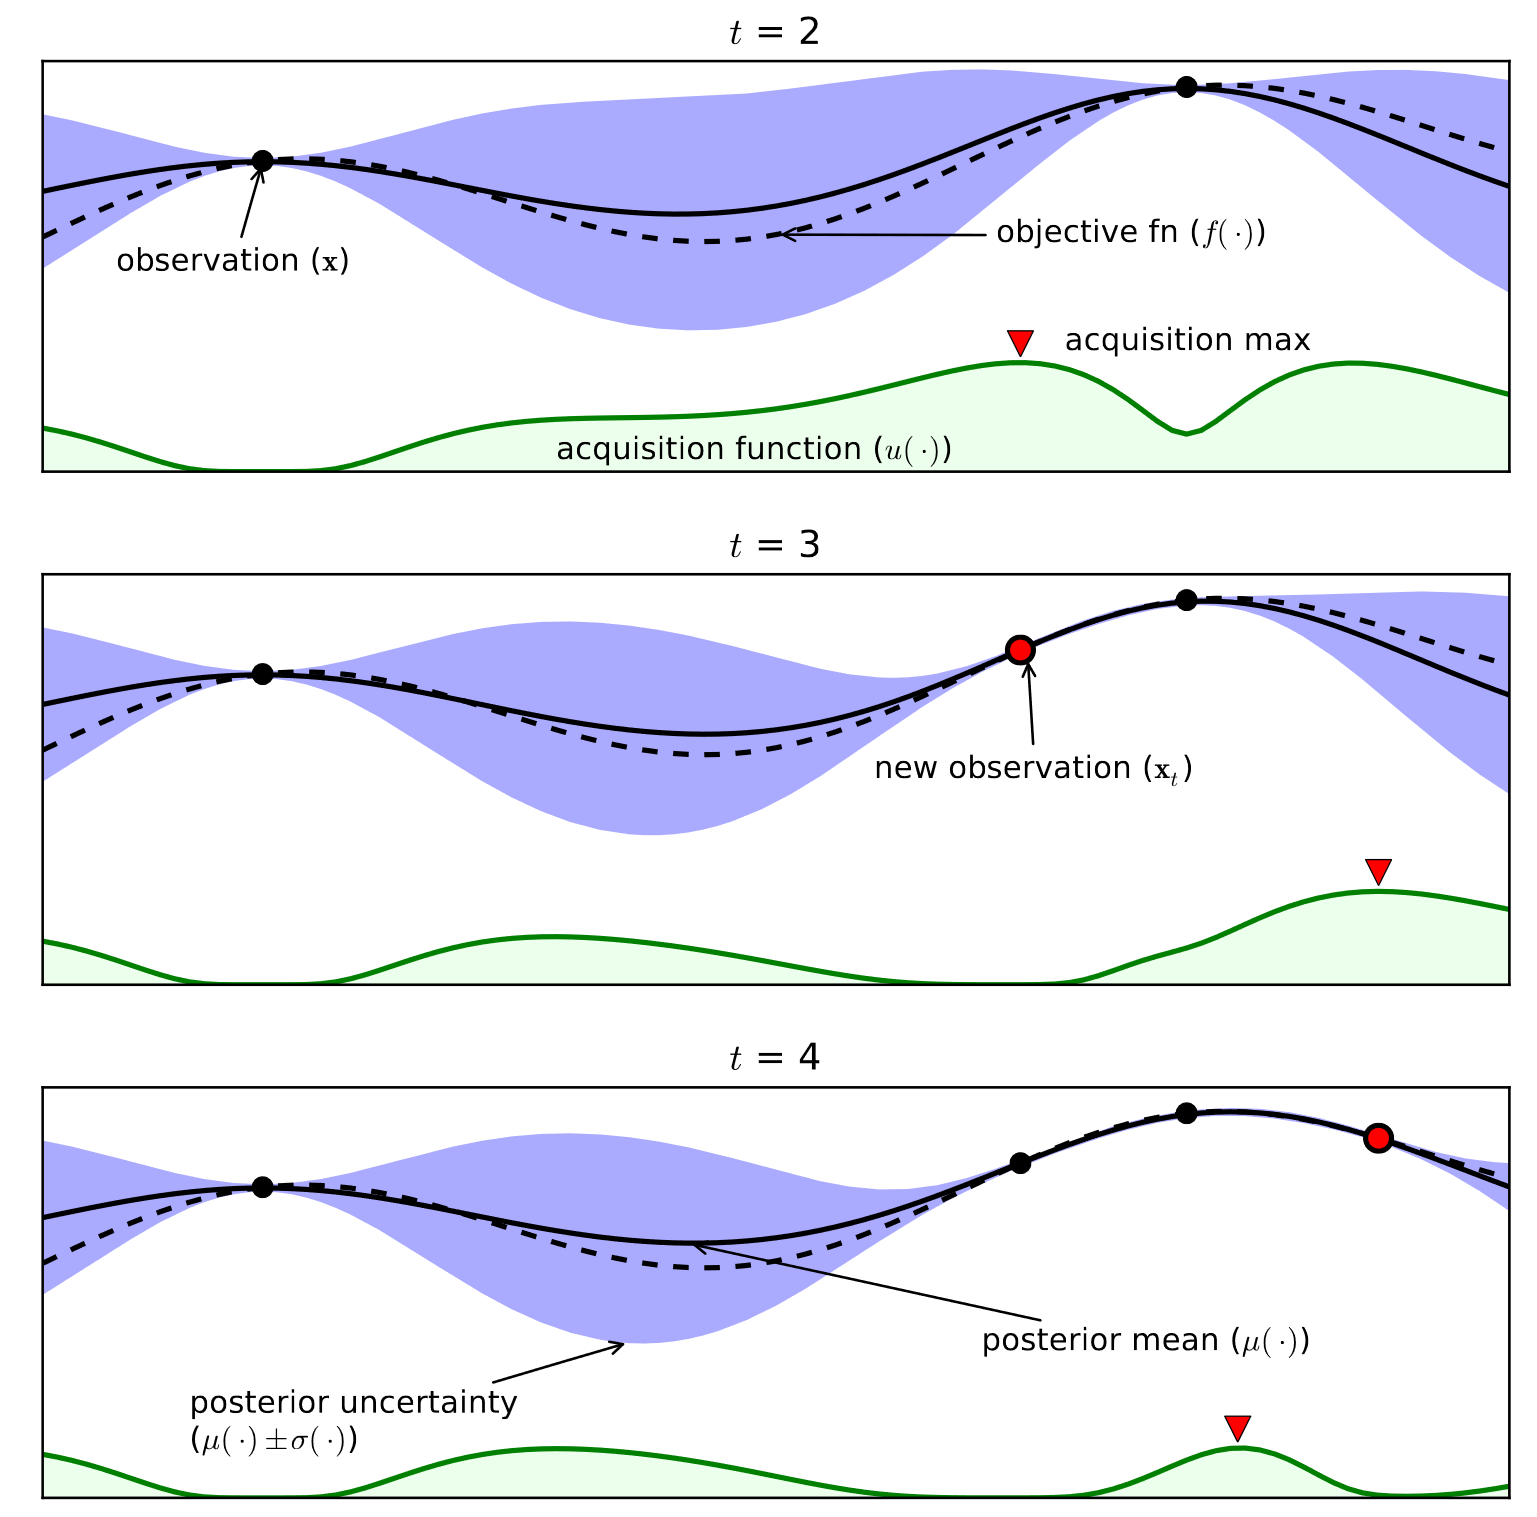
\includegraphics[width=\textwidth,height=0.5\textheight]{fig/bo.png}
\caption{Um exemplo do uso da otimização bayesiana em um problema de
design de brinquedo 1D.\label{bo}}
\end{figure}

A figura \ref{bo} mostram uma aproximação do processo Gaussiano (GP) da
função objetivo sobre quatro iterações dos valores amostrados da função
objetivo. A figura também mostra o função de aquisição nas parcelas
sombreadas mais baixas. A aquisição é alta onde o GP prevê um objetivo
elevado (exploração) e onde a incerteza de previsão é alta (exploração)
- áreas com os dois atributos são amostradas primeiro. Note que a área
no extrema esquerda permanece sem amostragem, como enquanto ele tem alta
incerteza, é (corretamente) previsto para oferecer pouca melhoria sobre
a mais alta observação.

A posteriori captura a apriori atualizada da função objetivo. Para que
uma amostra eficiente seja obtida é utilizado uma função de aquisição
para determinar o próximo ponto \(x_{t+1} \in A\). A decisão representa
um trade-off automático entre exploração (onde a função objetivo é muito
incerta) e exploração (tentando valores de \(x\) onde a função objetivo
deve ser alta). A optimização bayesiana tem como objetivo minimizar a
quantidade de interações necessárias para localizar o ponto máximo e
também se comporte bem em funções com múltiplos pontos de máximo.\\
~\\

A figura \ref{bo} representa um uma optimização de uma dimensão, onde é
iniciado com dois ponto aleatórios. A cada iteração, a função de
aquisição é maximizada para determinar o próximo ponto para a amostra da
função objetivo. A função de aquisição leva em consideração a média a
posteriori calculada para os pontos e a variância da previsão. E então é
amostrado o \(\operatorname{argmax}\) da função da função de aquisição,
o processo gaussiano é atualizado e o processo é repetido para os
próximos passos.\\

\newpage

\hypertarget{referuxeancias}{%
\chapter*{REFERÊNCIAS}\label{referuxeancias}}
\addcontentsline{toc}{chapter}{REFERÊNCIAS}

\hypertarget{refs}{}
\leavevmode\hypertarget{ref-bishop2012pattern}{}%
Bishop, Christopher M. 2012. ``Pattern Recognition and Machine Learning,
2006.'' \emph{Korean Society of Civil Engineers} 60 (1): 78--78.

\leavevmode\hypertarget{ref-chong2013introduction}{}%
Chong, Edwin KP, and Stanislaw H Zak. 2013. \emph{An Introduction to
Optimization}. Vol. 76. John Wiley \& Sons.

% ----------------------------------------------------------
% ELEMENTOS PÓS-TEXTUAIS
% ----------------------------------------------------------
\postextual

% ----------------------------------------------------------
% Referências bibliográficas
% ----------------------------------------------------------
\bibliography{bibliography.bibtex}

\printindex

\end{document}
